\documentclass[10pt]{article}
\usepackage[T1]{fontenc}
\usepackage[a4paper,textwidth=122mm,top=18mm,bottom=18mm]{geometry}
\usepackage{graphicx}
\usepackage{tikz}
\usepackage{pgfplots}
\usepackage{pgfplotstable}
\usetikzlibrary{arrows.meta,positioning}
\pgfplotsset{compat=1.18}
\definecolor{rtbdblue}{HTML}{0072B2}
\definecolor{rtbdorange}{HTML}{D55E00}
\definecolor{rtbdgreen}{HTML}{009E73}
\pgfplotsset{rtbdaxis/.style={width=0.95\linewidth,height=0.63\linewidth,
  tick label style={font=\small},label style={font=\small},
  legend style={font=\scriptsize,draw=none,fill=white},
  axis line style={thin},tick align=outside,grid=major,
  grid style={black!12},scaled ticks=false}}
\providecommand{\rtbddatadir}{outputs/figure_data}

\setlength{\parindent}{0pt}
\pgfplotstableread[col sep=comma]{
fleet,random,lwt,nearest
4,1356.6666666666667,1139.6666666666667,1368.0
5,1423.6666666666667,1412.3333333333333,1424.6666666666667
6,1424.6666666666667,1425.0,1425.0
}\rtbdTableb
\pgfplotstableread[col sep=comma]{
fleet,random,lwt,nearest
4,1356.6666666666667,1139.6666666666667,1368.0
5,1423.6666666666667,1412.3333333333333,1424.6666666666667
6,1424.6666666666667,1425.0,1425.0
}\rtbdTablec
\pgfplotstableread[col sep=comma]{
fleet,random,lwt,nearest
4,1356.6666666666667,1139.6666666666667,1368.0
5,1423.6666666666667,1412.3333333333333,1424.6666666666667
6,1424.6666666666667,1425.0,1425.0
}\rtbdTabled
\pgfplotstableread[col sep=comma]{
run,fleet,production_utilization,transport_persistence,wp_persistence,regime,congestion,throughput
411,4,0.8923761111111111,0.8333333333333334,0.20833333333333334,transport,0,1296
412,4,0.7002065972222222,0.9583333333333334,0.0,transport,0,1013
413,4,0.8994100231481481,0.875,0.08333333333333333,transport,0,1308
422,4,0.8414810300925926,0.9583333333333334,0.08333333333333333,transport,0,1223
432,4,0.8141511111111112,0.9583333333333334,0.0,transport,1,1183
}\rtbdTablee
\pgfplotstableread[col sep=comma]{
run,fleet,production_utilization,transport_persistence,wp_persistence,regime,congestion,throughput
431,4,0.9288448726851852,0.8333333333333334,0.375,mixed,1,1352
433,4,0.9448653125,0.75,0.4583333333333333,mixed,1,1374
}\rtbdTablef
\pgfplotstableread[col sep=comma]{
run,fleet,production_utilization,transport_persistence,wp_persistence,regime,congestion,throughput
532,5,0.9568542129629629,0.7083333333333334,0.4583333333333333,mixed,1,1392
}\rtbdTableg
\pgfplotstableread[col sep=comma]{
run,fleet,production_utilization,transport_persistence,wp_persistence,regime,congestion,throughput
421,4,0.9777869328703703,0.0,0.7083333333333334,production,0,1422
423,4,0.9777869328703703,0.0,0.625,production,0,1422
}\rtbdTableh
\pgfplotstableread[col sep=comma]{
run,fleet,production_utilization,transport_persistence,wp_persistence,regime,congestion,throughput
511,5,0.9802461458333334,0.0,0.6666666666666666,production,0,1425
512,5,0.9777869328703703,0.0,0.7083333333333334,production,0,1422
513,5,0.9802461458333334,0.0,0.7083333333333334,production,0,1425
521,5,0.9793846296296296,0.0,0.75,production,0,1424
522,5,0.9785768171296296,0.0,0.7083333333333334,production,0,1423
523,5,0.9803606597222222,0.0,0.625,production,0,1425
531,5,0.9777869212962963,0.0,0.7083333333333334,production,1,1422
533,5,0.9794562962962963,0.0,0.7916666666666666,production,1,1424
}\rtbdTablei
\pgfplotstableread[col sep=comma]{
run,fleet,production_utilization,transport_persistence,wp_persistence,regime,congestion,throughput
611,6,0.9812221296296296,0.0,0.6666666666666666,production,0,1426
612,6,0.981222175925926,0.0,0.7083333333333334,production,0,1426
613,6,0.9820174189814814,0.0,0.7083333333333334,production,0,1427
621,6,0.9812221180555556,0.0,0.75,production,0,1426
622,6,0.9802461226851852,0.0,0.7083333333333334,production,0,1425
623,6,0.980360613425926,0.0,0.7916666666666666,production,0,1425
631,6,0.9777869675925925,0.0,0.7083333333333334,production,1,1422
632,6,0.9793846412037037,0.0,0.7083333333333334,production,1,1424
633,6,0.9785947337962962,0.0,0.625,production,1,1423
}\rtbdTablej
\pgfplotstableread[col sep=comma]{
run,fleet,production_utilization,transport_persistence,wp_persistence,regime,congestion,throughput
412,4,0.8707915023148148,0.9583333333333334,0.0,transport,0,1013
}\rtbdTableba
\pgfplotstableread[col sep=comma]{
run,fleet,production_utilization,transport_persistence,wp_persistence,regime,congestion,throughput
411,4,0.9510439143518519,0.8333333333333334,0.20833333333333334,mixed,0,1296
413,4,0.9549548078703703,0.875,0.08333333333333333,mixed,0,1308
422,4,0.9302572673611111,0.9583333333333334,0.08333333333333333,mixed,0,1223
431,4,0.9673435775462963,0.8333333333333334,0.4166666666666667,mixed,1,1352
432,4,0.9225686817129629,0.9583333333333334,0.041666666666666664,mixed,1,1183
433,4,0.9742880914351851,0.75,0.4583333333333333,mixed,1,1374
}\rtbdTablebb
\pgfplotstableread[col sep=comma]{
run,fleet,production_utilization,transport_persistence,wp_persistence,regime,congestion,throughput
532,5,0.9813674988425926,0.7083333333333334,0.4583333333333333,mixed,1,1392
}\rtbdTablebc
\pgfplotstableread[col sep=comma]{
run,fleet,production_utilization,transport_persistence,wp_persistence,regime,congestion,throughput
421,4,0.9897768738425926,0.0,0.75,production,0,1422
423,4,0.9890648923611111,0.0,0.6666666666666666,production,0,1422
}\rtbdTablebd
\pgfplotstableread[col sep=comma]{
run,fleet,production_utilization,transport_persistence,wp_persistence,regime,congestion,throughput
511,5,0.9911957013888889,0.0,0.7083333333333334,production,0,1425
512,5,0.9906562025462963,0.0,0.75,production,0,1422
513,5,0.9914271782407408,0.0,0.75,production,0,1425
521,5,0.9908086550925926,0.0,0.7916666666666666,production,0,1424
522,5,0.9905072025462963,0.0,0.75,production,0,1423
523,5,0.9909792164351852,0.0,0.6666666666666666,production,0,1425
531,5,0.9891906157407407,0.0,0.75,production,1,1422
533,5,0.9905198993055555,0.0,0.8333333333333334,production,1,1424
}\rtbdTablebe
\pgfplotstableread[col sep=comma]{
run,fleet,production_utilization,transport_persistence,wp_persistence,regime,congestion,throughput
611,6,0.9912692233796296,0.0,0.7083333333333334,production,0,1426
612,6,0.9911688055555555,0.0,0.75,production,0,1426
613,6,0.9912087511574074,0.0,0.75,production,0,1427
621,6,0.991194994212963,0.0,0.7916666666666666,production,0,1426
622,6,0.9913622210648149,0.0,0.75,production,0,1425
623,6,0.9911041319444445,0.0,0.8333333333333334,production,0,1425
631,6,0.9897463541666667,0.0,0.75,production,1,1422
632,6,0.9899254629629629,0.0,0.75,production,1,1424
633,6,0.9901460462962963,0.0,0.6666666666666666,production,1,1423
}\rtbdTablebf
\pgfplotstableread[col sep=comma]{
fleet,forward,backward,bidirectional
4,0.0,0.0,7.077761959876544
5,0.0,0.0,7.184051697530864
6,0.0,0.0,6.254206275720165
}\rtbdTablebg
\pgfplotstableread[col sep=comma]{
fleet,forward,backward,bidirectional
4,0.0,0.0,7.077761959876544
5,0.0,0.0,7.184051697530864
6,0.0,0.0,6.254206275720165
}\rtbdTablebh
\pgfplotstableread[col sep=comma]{
fleet,forward,backward,bidirectional
4,0.0,0.0,7.077761959876544
5,0.0,0.0,7.184051697530864
6,0.0,0.0,6.254206275720165
}\rtbdTablebi
\begin{document}
\begin{center}\large RTBD reproducibility figures\end{center}
\textbf{Filtered completed-case reference.} The following figures reproduce
the completed-case input corpus. The raw-data comparison follows.
\begin{figure}[ht]\centering\begin{tikzpicture}
\begin{axis}[rtbdaxis,xlabel={AGV fleet size},ylabel={Completed products},
  xtick={4,5,6},xmin=3.9,xmax=6.1,ymin=1100,ymax=1460,legend pos=south east]
\addplot[rtbdblue,thick,mark=*] table[x=fleet,y=random,col sep=comma]{\rtbdTableb};
\addlegendentry{Random}
\addplot[rtbdorange,thick,dashed,mark=square*] table[x=fleet,y=lwt,col sep=comma]{\rtbdTablec};
\addlegendentry{Longest-Waiting-Time}
\addplot[rtbdgreen,thick,dashdotted,mark=triangle*] table[x=fleet,y=nearest,col sep=comma]{\rtbdTabled};
\addlegendentry{Nearest-Vehicle}
\end{axis}
\end{tikzpicture}

\caption{Throughput by fleet size and dispatch policy, averaged over the three driving directions.}\end{figure}
\begin{figure}[ht]\centering\begin{tikzpicture}
\begin{axis}[rtbdaxis,xlabel={Maximum production utilization},
  ylabel={Transport-pressure persistence},xmin=0.65,xmax=1.01,ymin=-0.035,ymax=1.04,
  xtick={0.7,0.8,0.9,1.0},ytick={0,0.25,0.5,0.75,1},
  legend style={at={(0.5,-0.27)},anchor=north,legend columns=3,font=\scriptsize,draw=none}]
\addplot[black!40,densely dotted,forget plot] coordinates {(0.9,-0.035) (0.9,1.04)};
\addplot[black!40,densely dotted,forget plot] coordinates {(0.65,0.5) (1.01,0.5)};
\addplot[only marks,rtbdorange,mark=*,mark size=2.5pt,forget plot] table[x=production_utilization,y=transport_persistence,col sep=comma]{\rtbdTablee};
\addplot[only marks,rtbdgreen,mark=*,mark size=2.5pt,forget plot] table[x=production_utilization,y=transport_persistence,col sep=comma]{\rtbdTablef};
\addplot[only marks,rtbdgreen,mark=square*,mark size=2.5pt,forget plot] table[x=production_utilization,y=transport_persistence,col sep=comma]{\rtbdTableg};
\addplot[only marks,rtbdblue,mark=*,mark size=2.5pt,forget plot] table[x=production_utilization,y=transport_persistence,col sep=comma]{\rtbdTableh};
\addplot[only marks,rtbdblue,mark=square*,mark size=2.5pt,forget plot] table[x=production_utilization,y=transport_persistence,col sep=comma]{\rtbdTablei};
\addplot[only marks,rtbdblue,mark=triangle*,mark size=2.5pt,forget plot] table[x=production_utilization,y=transport_persistence,col sep=comma]{\rtbdTablej};
\addlegendimage{only marks,mark=*,black}\addlegendentry{4 AGVs}
\addlegendimage{only marks,mark=square*,black}\addlegendentry{5 AGVs}
\addlegendimage{only marks,mark=triangle*,black}\addlegendentry{6 AGVs}
\addlegendimage{only marks,mark=*,rtbdorange}\addlegendentry{Transport pressure}
\addlegendimage{only marks,mark=*,rtbdgreen}\addlegendentry{Mixed pressure}
\addlegendimage{only marks,mark=*,rtbdblue}\addlegendentry{Production pressure}
\end{axis}
\end{tikzpicture}

\caption{RTBD evidence for all 27 filtered logs. Coincident markers can overlap. Colors show the computed regime; production pressure also requires Welding--Painting joint persistence. Dotted lines show the 0.90 saturation and 0.50 transport-persistence cutoffs.}\end{figure}
\clearpage
\textbf{Raw-data sensitivity.} All raw cases are included; unfinished
intervals are right-censored at the 24-hour observation boundary.
\renewcommand{\rtbddatadir}{outputs/figure_data/raw}
\begin{figure}[ht]\centering\begin{tikzpicture}
\begin{axis}[rtbdaxis,xlabel={Maximum production utilization},
  ylabel={Transport-pressure persistence},xmin=0.65,xmax=1.01,ymin=-0.035,ymax=1.04,
  xtick={0.7,0.8,0.9,1.0},ytick={0,0.25,0.5,0.75,1},
  legend style={at={(0.5,-0.27)},anchor=north,legend columns=3,font=\scriptsize,draw=none}]
\addplot[black!40,densely dotted,forget plot] coordinates {(0.9,-0.035) (0.9,1.04)};
\addplot[black!40,densely dotted,forget plot] coordinates {(0.65,0.5) (1.01,0.5)};
\addplot[only marks,rtbdorange,mark=*,mark size=2.5pt,forget plot] table[x=production_utilization,y=transport_persistence,col sep=comma]{\rtbdTableba};
\addplot[only marks,rtbdgreen,mark=*,mark size=2.5pt,forget plot] table[x=production_utilization,y=transport_persistence,col sep=comma]{\rtbdTablebb};
\addplot[only marks,rtbdgreen,mark=square*,mark size=2.5pt,forget plot] table[x=production_utilization,y=transport_persistence,col sep=comma]{\rtbdTablebc};
\addplot[only marks,rtbdblue,mark=*,mark size=2.5pt,forget plot] table[x=production_utilization,y=transport_persistence,col sep=comma]{\rtbdTablebd};
\addplot[only marks,rtbdblue,mark=square*,mark size=2.5pt,forget plot] table[x=production_utilization,y=transport_persistence,col sep=comma]{\rtbdTablebe};
\addplot[only marks,rtbdblue,mark=triangle*,mark size=2.5pt,forget plot] table[x=production_utilization,y=transport_persistence,col sep=comma]{\rtbdTablebf};
\addlegendimage{only marks,mark=*,black}\addlegendentry{4 AGVs}
\addlegendimage{only marks,mark=square*,black}\addlegendentry{5 AGVs}
\addlegendimage{only marks,mark=triangle*,black}\addlegendentry{6 AGVs}
\addlegendimage{only marks,mark=*,rtbdorange}\addlegendentry{Transport pressure}
\addlegendimage{only marks,mark=*,rtbdgreen}\addlegendentry{Mixed pressure}
\addlegendimage{only marks,mark=*,rtbdblue}\addlegendentry{Production pressure}
\end{axis}
\end{tikzpicture}

\caption{Raw-log evidence. Four four-AGV configurations change from transport pressure with low completed-case production exposure to mixed pressure. Throughput is unchanged.}\end{figure}
\renewcommand{\rtbddatadir}{outputs/figure_data}
\begin{figure}[ht]\centering\begin{tikzpicture}
\begin{axis}[rtbdaxis,xlabel={AGV fleet size},ylabel={Blocked fleet capacity (\%)},
  xmin=3.9,xmax=6.1,ymin=-0.3,ymax=8,xtick={4,5,6},legend pos=north east]
\addplot[rtbdblue,thick,mark=*,mark options={fill=white},mark size=3pt] table[x=fleet,y=forward,col sep=comma]{\rtbdTablebg};
\addlegendentry{Forward}
\addplot[rtbdgreen,thick,dashed,mark=x,mark size=2pt] table[x=fleet,y=backward,col sep=comma]{\rtbdTablebh};
\addlegendentry{Backward}
\addplot[rtbdorange,thick,dashdotted,mark=triangle*] table[x=fleet,y=bidirectional,col sep=comma]{\rtbdTablebi};
\addlegendentry{Bidirectional}
\end{axis}
\end{tikzpicture}

\caption{Supplementary filtered-log figure: blocked fleet-capacity time by fleet size and direction. Forward and Backward are both zero.}\end{figure}
\clearpage
\textbf{Original native pipeline.}
\begin{figure}[ht]\centering\resizebox{\linewidth}{!}{%
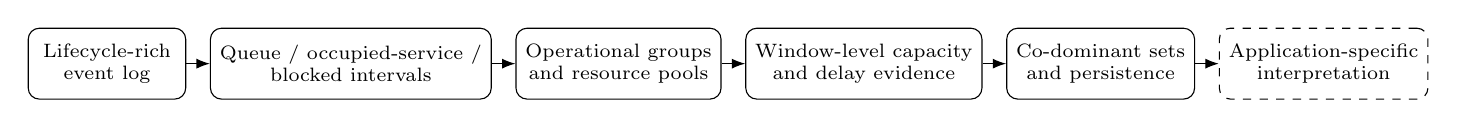
\begin{tikzpicture}[
    node distance=3mm,
    every node/.style={font=\scriptsize,align=center},
    box/.style={
        draw,
        rounded corners,
        minimum width=20mm,
        minimum height=9mm,
        inner sep=1.2mm
    },
    interp/.style={
        draw,
        dashed,
        rounded corners,
        minimum width=20mm,
        minimum height=9mm,
        inner sep=1.2mm
    },
    arr/.style={-{Latex[length=1.7mm]},thin}
]
\node[box] (log) {Lifecycle-rich\\event log};
\node[box,right=of log] (int) {Queue / occupied-service /\\blocked intervals};
\node[box,right=of int] (pool) {Operational groups\\and resource pools};
\node[box,right=of pool] (evid) {Window-level capacity\\and delay evidence};
\node[box,right=of evid] (set) {Co-dominant sets\\and persistence};
\node[interp,right=of set] (regime) {Application-specific\\interpretation};

\draw[arr] (log)--(int);
\draw[arr] (int)--(pool);
\draw[arr] (pool)--(evid);
\draw[arr] (evid)--(set);
\draw[arr] (set)--(regime);
\end{tikzpicture}
}

\caption{Generic measurement layer and application-specific interpretation, retained from the supplied manuscript.}\end{figure}
\end{document}
